\section{Overall Landscape of Satellite Embeddings}

\subsection{Why an embedding-centered review?}

Most existing remote sensing foundation model surveys are organized around pretraining paradigms, modality combinations, or downstream tasks. That is useful for describing the broader field, but it is not the most natural entry point for practitioners. In operational use, the object that is actually reused is usually an embedding: a pooled scene vector, a dense token grid, an annual embedding field, or a joint multimodal latent space. This review therefore starts from the reusable representation layer rather than from the training recipe alone.

\subsection{What is a satellite embedding?}

In this review, a satellite embedding is a reusable latent representation derived from satellite or related Earth observation data and intended to support multiple downstream tasks beyond the pretraining objective. This definition intentionally includes both on-the-fly encoder outputs and precomputed embedding products. It excludes purely task-specific logits or handcrafted indices unless they are explicitly repackaged as a transferable representation layer.

Four representation forms appear repeatedly in the current literature:

\begin{enumerate}[leftmargin=1.4em]
  \item \textbf{Pooled scene vectors}, commonly exposed by transformer encoders for classification, regression, or similarity search.
  \item \textbf{Dense token grids}, which preserve local spatial structure and can support segmentation or dense retrieval.
  \item \textbf{Annual embedding fields}, where the representation is served as a spatial product rather than recomputed at inference time.
  \item \textbf{Joint multimodal spaces}, where the embedding aligns imagery with text, metadata, or additional sensor streams.
\end{enumerate}

\begin{figure}[t]
  \centering
  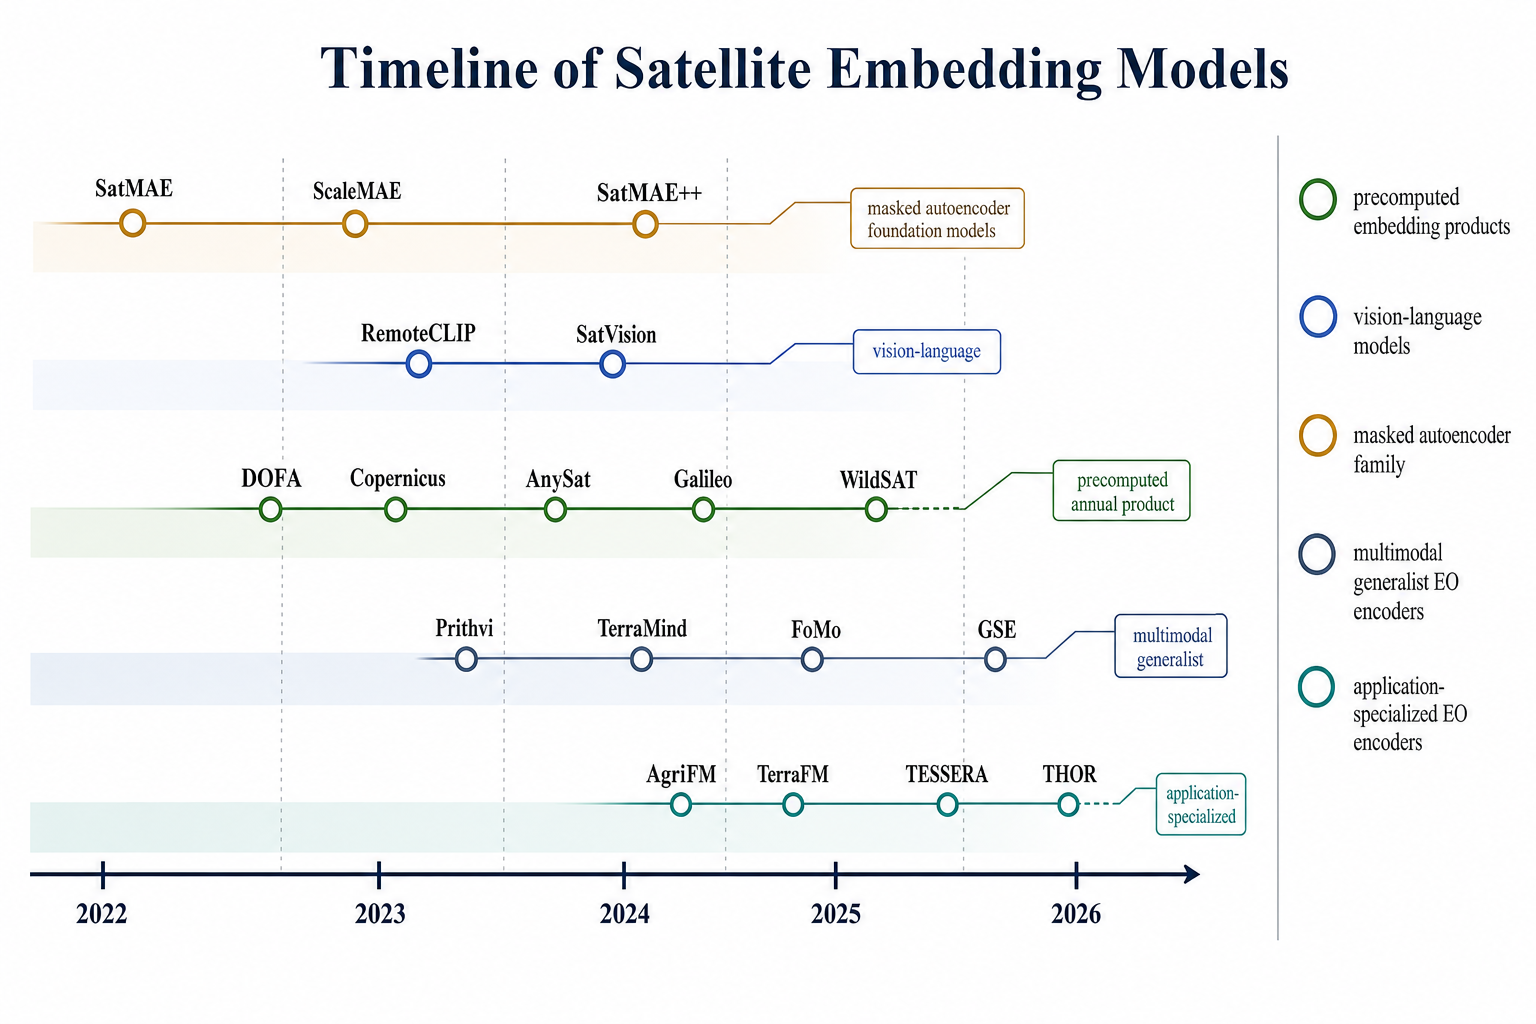
\includegraphics[width=\textwidth]{fig04_model_timeline_gptimage2_20260502.png}
  \caption{Model timeline view for the satellite embedding landscape. The figure emphasizes how precomputed products, masked autoencoder lineages, multimodal generalists, and application-specific encoders accumulate over time rather than appearing as a single homogeneous wave.}
  \label{fig:model-timeline}
\end{figure}

\subsection{Field evolution and major design axes}

For a remote sensing review, the overall story should appear before the detailed taxonomy. The field has evolved from early optical and masked-reconstruction pipelines toward broader multimodal, temporal, vision-language, and productized embedding systems. Figure~\ref{fig:model-timeline} provides this overall chronological view, which is easier for readers to absorb than a flat list of models.

We organize the literature along three orthogonal axes.

\paragraph{Model family.}
The first axis groups models by how the representation is learned and exposed: precomputed embedding products \citep{gse,tessera,copernicus}, vision-language systems \citep{remoteclip,wildsat}, masked autoencoder derivatives \citep{satmae,satmaepp,scalemae}, multimodal generalist encoders \citep{anysat,galileo,prithvi,terrafm,terramind,dofa}, and application-specialized Earth observation encoders \citep{agrifm,fomo,thor,satvision}.

\paragraph{Data and modality.}
The second axis captures the sensing substrate. Current models differ in optical-only versus optical-plus-SAR support, single-scene versus time-series modeling, fixed spectral assumptions versus wavelength-aware adaptation, and fine-resolution surface imagery versus coarse-resolution all-sky or atmosphere-linked sensing.

\paragraph{Deployment mode.}
The third axis separates systems that run a neural encoder at query time from systems that distribute the embedding directly as a product. This distinction is central for benchmarking because it changes runtime, storage, temporal flexibility, and failure modes. A precomputed product may offer extremely fast access but less temporal control, while an on-the-fly encoder may provide higher flexibility at the cost of data loading and GPU latency.

\begin{figure}[t]
  \centering
  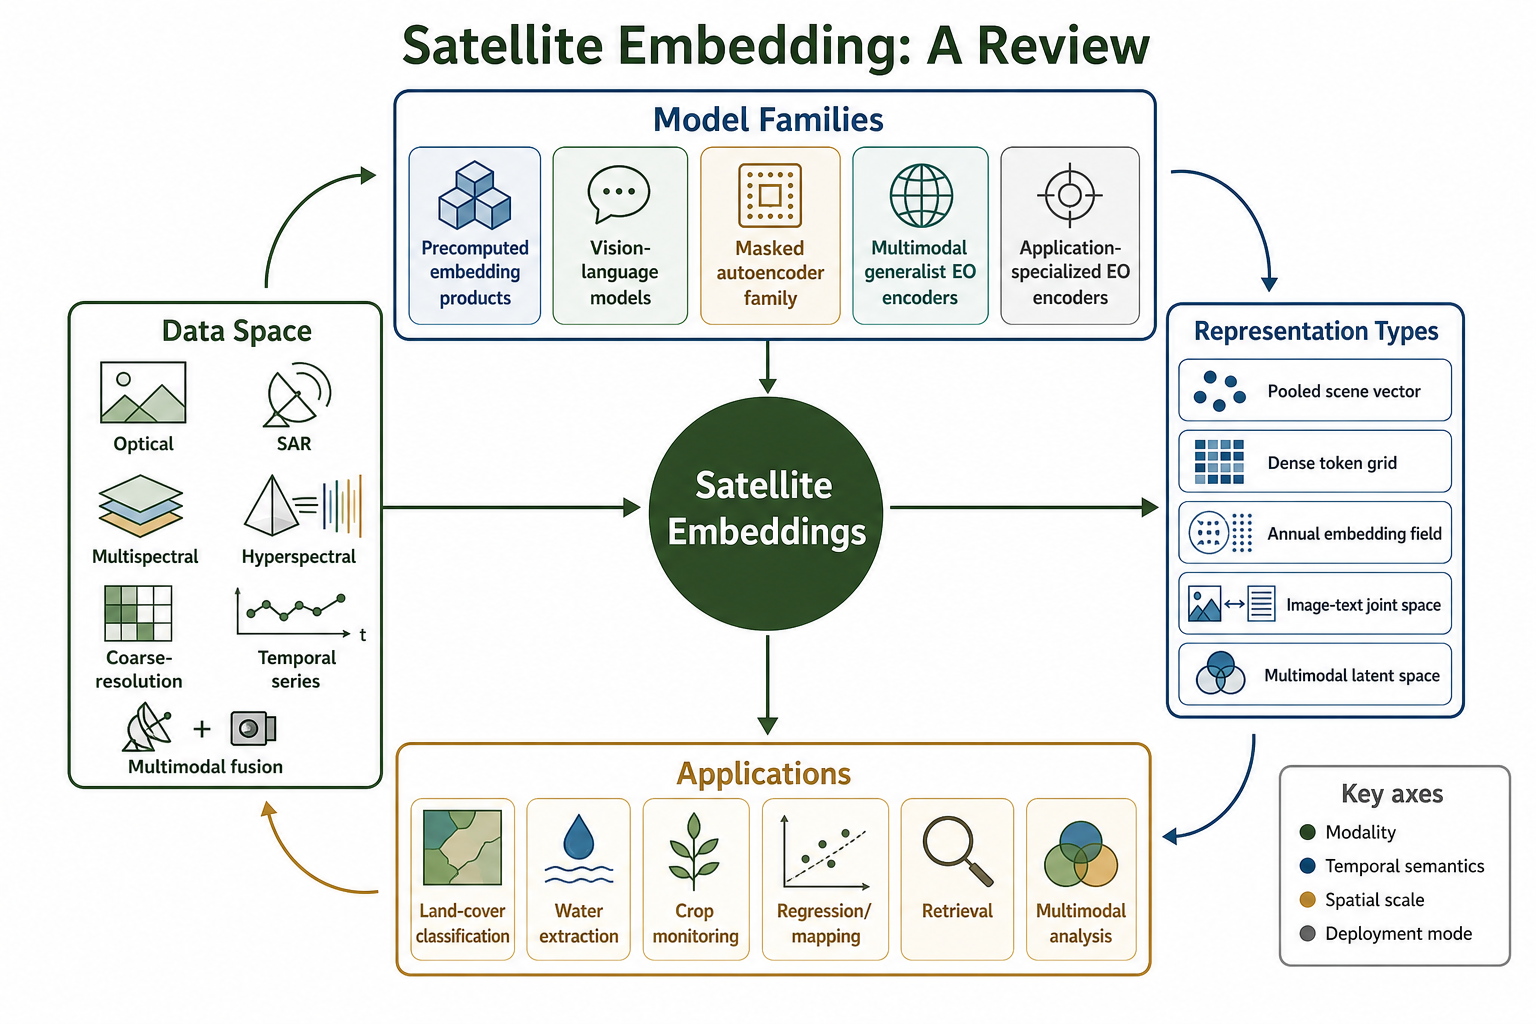
\includegraphics[width=\textwidth]{fig01_taxonomy_concept_map_gptimage2_20260502.png}
  \caption{Conceptual map of the satellite embedding landscape. The review is structured around four linked components: data space, model family, representation type, and downstream application. This framing is intentionally embedding-centered rather than checkpoint-centered.}
  \label{fig:taxonomy-concept-map}
\end{figure}

\subsection{Scope of this review}

An embedding-centered review should not simply relabel all remote sensing foundation models as satellite embeddings. Instead, the central question is whether the representation can serve as a general interface for downstream use. This criterion explains why annual products such as GSE and TESSERA belong in the same discussion as encoder checkpoints such as SatMAE++, AnySat, or TerraFM. All of them provide a transferable representation layer, but they differ sharply in spatial scale, temporal semantics, and deployment assumptions. Figure~\ref{fig:taxonomy-concept-map} summarizes this review logic in one diagram.
